\documentclass[
  % Replace twoside with oneside if you are printing your thesis on a single side
  % of the paper, or for viewing on screen.
  %oneside,
  oneside,
  11pt, a4paper,
  footinclude=true,
  headinclude=true,
  cleardoublepage=empty
]{article}

\usepackage{lipsum}
\usepackage{amsmath}
\usepackage{amsthm}
\usepackage{acronym}
\usepackage{hyperref}
\usepackage{graphicx}
\usepackage{apacite}
\usepackage[utf8]{inputenc}
\graphicspath{{images/}}

\title{Virtour: Telepresence system for remotely-operated building tours}
\author{Patricio Lankenau\\
        University of Texas at Austin, Austin, Texas\\
        patricio.lankenau@utexas.edu\\}
\date{}

\begin{document}

\maketitle

\tableofcontents
\newpage

\section{Introduction}

The University of Texas at Austin has a constant stream of visitors and tours
of the beautiful campus. Of special interest to us are the large number of
tours given at our computer science building. The tour guests range in ages and
backgrounds, and tend to be prospective students to both undergraduate and
gradate programs, or visiting faculty. Unfortunately, there is a large
population of prospective students that are unable to physically come to our
campus and are thus unable to partake in the conventional tours.

This is why we designed Virtour. Virtour is a public facing system for
teleoperated building tours. Virtour builds on the existing Building-Wide
Intelligence autonomous robot platform and is designed to keep the robots and
any humans involved safe.  It utilizes the lab's autonomous wheeled robots
which can localize, navigate, and perform tasks without human intervention for
long periods of time.

Through the use of modern web and robot technologies it allows untrained public
users to remotely control our robots in what we call a virtual tour. Our system
is created to balance external control abilities while maintaining our rigorous
standard of safety and security for the robots and people involved. As such it
gives the user control of what the robot is doing, while simultaneously using
existing the autonomous navigation capabilities and obstacle avoidance to
provide the user with shared autonomy.

\section{Related Work}

Web-based tours have been an active area of research in the past. The earliest
virtual tour system was built to serve as a museum tour guide in 1998 by
\cite{burgard1998}. Their robot, Rhino, operated mainly as a physically
interactive tour guide that museum visitors could approach and request tours
from, but also supported ocasionaly web-based tours where online visitors could
vote on certain tours to use. Their web-based interface provided images from
the on-board camera as well as static cameras placed throughout the museum, and
allowed the user to download a Java applet to see real-time information. Web
control was limited to voting on a desired tour (from a pre-programmed list)
and viewing the robot's image stream.

Later work introduced a second-generation museum tour-guide robot by
\cite{thrun1999} named Minerva, which improved on the work done by Burgard.
Most of their improvements were around localization, mapping, SLAM, and HRI.
They improved the virtual tour interface by allowing arbitrary selection of
navigation goals, rather than a pre-selected list. However, web control was
still limited and their real-time information display required the download of
a Java web-applet.

\cite{km2004} al developed Jinny in 2004, which was yet another autonomous
tour-guide robot. Their relevant contribution was the upgraded web-based
interface which allowed the user to interact with the natural language parsing
system and ask questions, as well as request actions. Their system was built
using Java, ActiveX, and Javascript, all of which require special installation
on part of the end user to use.

More recent work virtual tour and telepresence systems were built in 2007
\cite{michaud2007} and in 2013 \cite{kusu2013}. Kusu, et al's system is relevant
because it was designed to provide campus tours.

Virtour differs from these related works in various ways. The first is that
virtour's main purpose is to be a telepresence tour system, and thus gives web
visitors priority in controlling the robot (unlike Rhino or Minerva which only
ocasionally allow web control). Our system is unique in that it uses
only modern web standards and does not require the end-user to download any
extra software (eg: Java, ActiveX). Thus virtour can be truly portable and
accessed from any computer, tablet, or mobile device. Virtour is also
unique in that it provides the end-user with real-time video feedback and
information about the robot. For example, the robot's position will be updated
on the website in real-time without requiring any additional simulation
software. Furthermore, the user's actions are performed in real-time and the
results are shown almost immediately. So if a user request the robot to rotate,
he or she will be able to see the robot's camera feed update instantly.  As
part of virtour's goal of ease of use, it uses bandwidth scaling of video
streaming to reduce the quality of the video according to the end-user's
internet connection. Finally, virtour is novel because it provides the end-user
with a wide variety of ways of interacting with the robot. Rather than just
providing navigation and video streaming, it allows the user to deliver spoken
messages and perform tasks.

\section{Building Wide Intelligence}

Virtour is a part of the Building Wide Intelligence (BWI) project, which aims
to develop fully autonomous mobile robots. The goal is to have these robots be
permanent inhabitants of UT's Computer Science departmental building. BWI
focuses on the intersection of Artificial Intelligence and Robotics, and works
on creating robots that are useful as research platforms, as well service
robots to help the humans in the building.

Virtour runs on the BWI segbot robot platform. Our lab has four currently
active robots. Three of which are based on the older generation hardware and
software. We have one version 3 robot which has been our pilot as we transition
all our robots to new hardware and software. Although virtour supports both
versions, and will adapt its features accordingly, it is mostly used on the
latest generation so that is what is described.

\begin{figure}
\centering
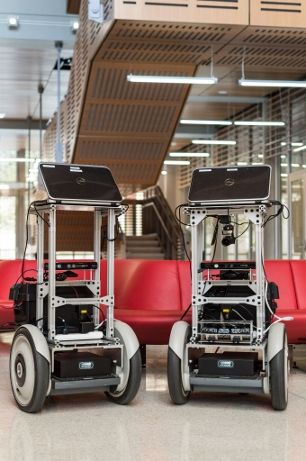
\includegraphics[height=2in]{bwi}
\caption{Two of our second generation BWI robots}
\end{figure}

\subsection{Hardware Platform}

All of our robots are powered by the Segway Robotics Mobility Platform (RMP).
Our latest generation robot uses a more advanced RMP version which comes with
two integrated lithium-ion batteries. The frame was designed in-house and
supports a wide array of sensors. For navigation, localization, and obstacle
avoidance, we use a Velodyne Puck lidar. Point clouds (3D voxel map) and RGB
data are provided by a Microsoft Kinect sensor. Our latest generation robots
also have an additional laser range finder to compensate for the lidar's blind
spots. The robot is equipped with a custom-built computer which runs Ubuntu
14.04. The computer is powered by the RMPs battery, thus removing the need for
an external car battery (which was present in our version 2 robots).  The
battery life on a running robot is approximately 6 hours when actively using
the base, and 10 when stationary.

\subsection{Software Stack}

Our robots are powered by the Robot Operating System (ROS), which provides us
with the infrastructure to run as a distributed node system. It provides the
messaging framework to connect all the different components. ROS also provides
us with access to many community packages such as device drivers, navigation
implementations, and planning systems.

Our navigation stack starts out with the logical planner, which uses Answer Set
Programming (ASP) (TODO: cite ASP paper) to plan and describe the environment
(eg: which corridors connect with which hallways, and which doors are open). It
then moves to the logical navigator which uses the previous laser readings and
what it knows about the environment to create the navigation plan. Finally, the
local planner uses the immediate sensor readings to send commands to the segway
base and avoid any obstacles.

All of our software is open source and freely available
online\footnote{\url{http://github.com/utexas-bwi}}.

\section{The Web Client}

\begin{figure}
\centering
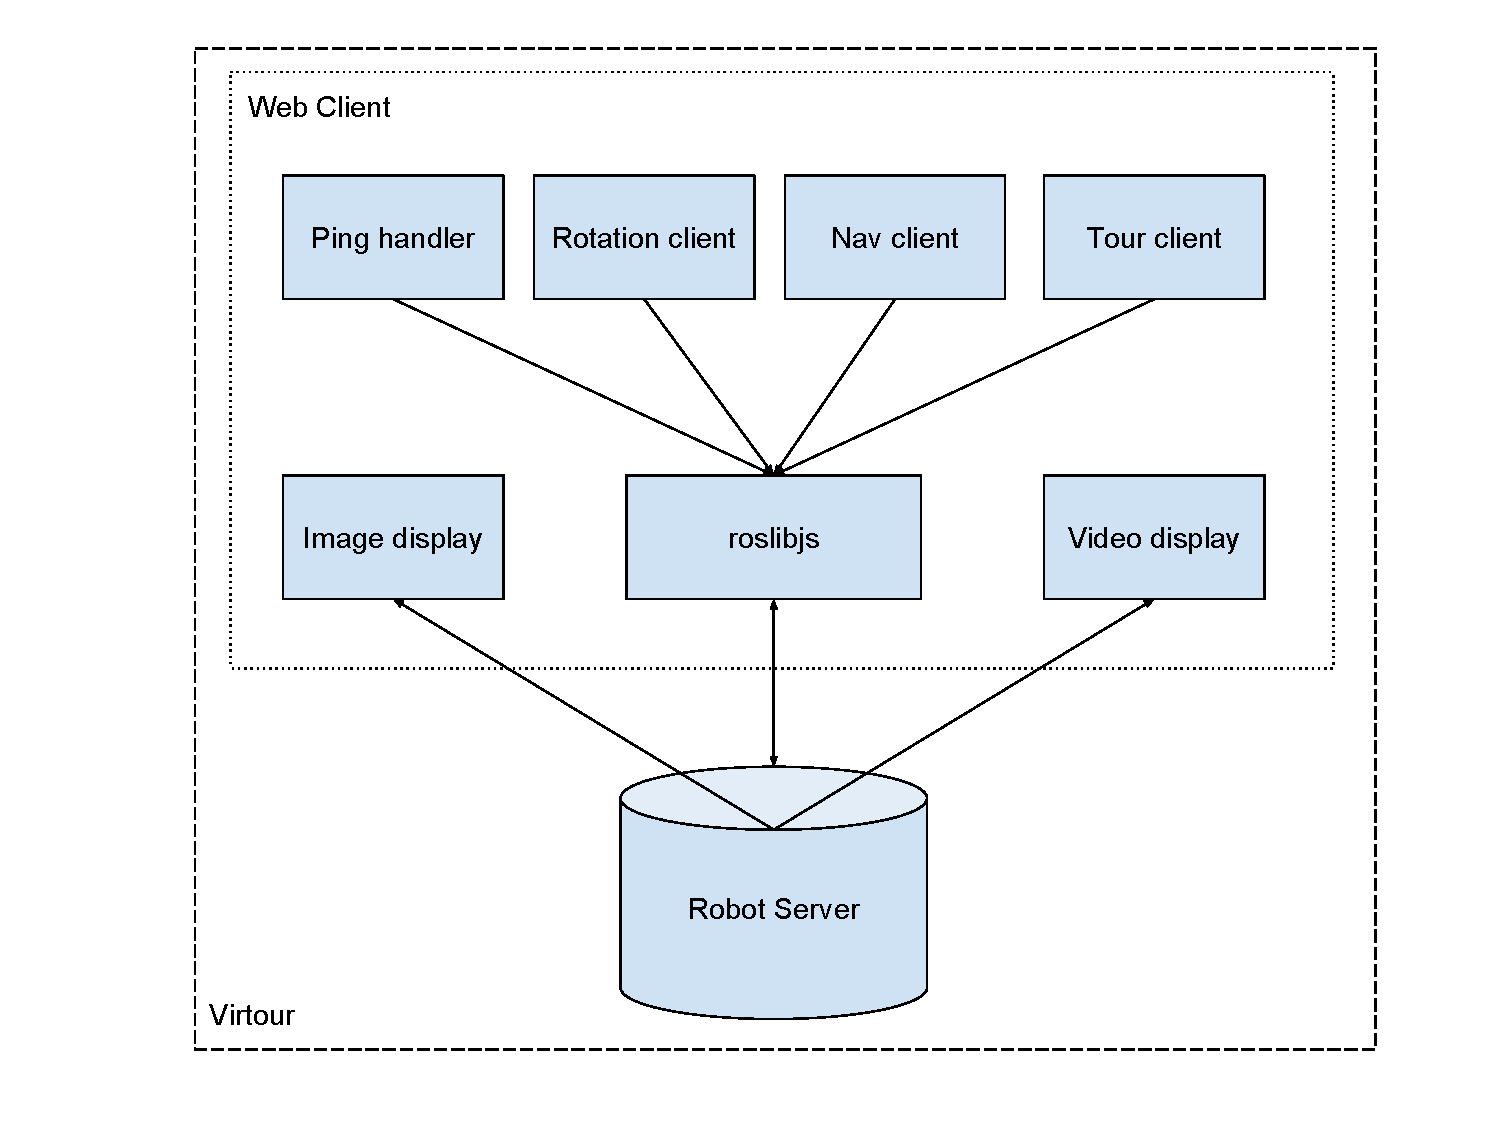
\includegraphics[width=3in]{virtour_client}
\caption{Overview of the virtour client structure and hierarchy}
\end{figure}

Virtour consists of two platforms, the user facing client, and the server and
associated software that runs on the robots. The user client is accessible from
a web browser and is built using web 2.0 technologies to adhere to modern web
development trends and simultaneously support as many platforms as possible. We
decided to use a web-based client because of the increasing prominence of web
browsers in people's lives. Furthermore, a web based approach means that our
end-users do not have to install any additional software to connect with or use
the robots, thus reducing the friction for trying our service.

\subsection{Modern Approach}

The web client is designed to be simple and functional while still being
aesthetically pleasing to end users. It uses a grid system powered by the
popular front-end library, Bootstrap 2.0 (TODO: cite), to create a fully
responsive web layout. This allows us to support any web-powered platform (eg:
mobile devices, tablets, and computers) by making the website scale and
re-organize based on the specifications of the device.

When a user first visits our website, he or she is greeted by a list of our
currently active and available robots (more on server implementation later).
Each robot is represented by a name and associated picture \footnote{All of our
robots are named after Futurama characters}. From here our user can select a
robot to connect to (by clicking on the robot's name or image) to initiate a
virtual tour session. When the user clicks on the robot, the web client will
initiate a request to the specified robot requesting a tour session.

Tour sessions can be either led or spectated. When spectating the user has no
control over the robot but can see the video stream, robot status, and track
the location of the robot along the map in real time. A led tour is one one in
which the user can actively instruct the robot to perform operations. Each tour
can have at most one leader, but no limit on the number of spectators. We built
virtour this way to ensure there is a consistent leader experience (to avoid tour
contention by multiple users), and for security reasons, since we can control
whether a leader is allowed or not. If the tour has no existing leader and
tours are allowed then a visiting user can elect to become tour leader by
pressing the ``Become Leader'' button. Upon success, it will present the user
with the leader UI.

\begin{figure}
\centering
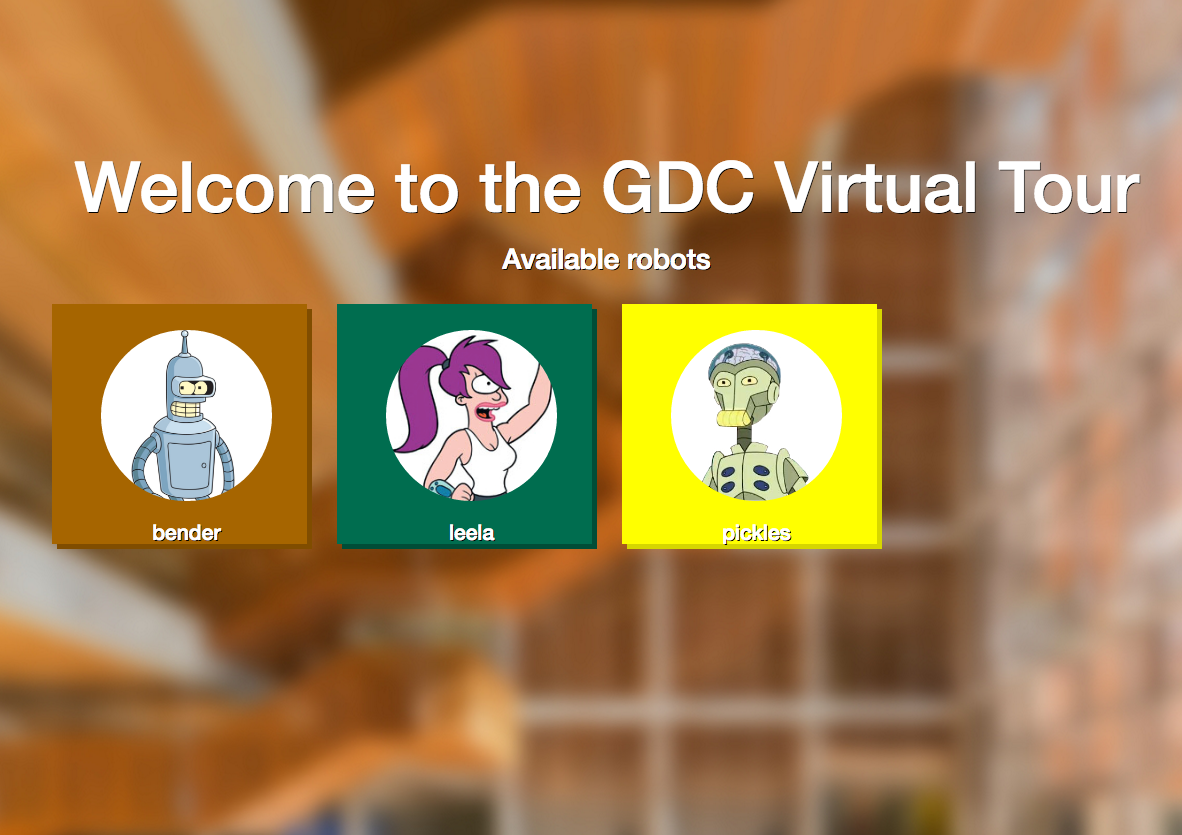
\includegraphics[width=3in]{tour_homepage}
\caption{Landing page whenever someone visits the home page}
\end{figure}

\subsection{Leader UI}

\begin{figure}
\centering
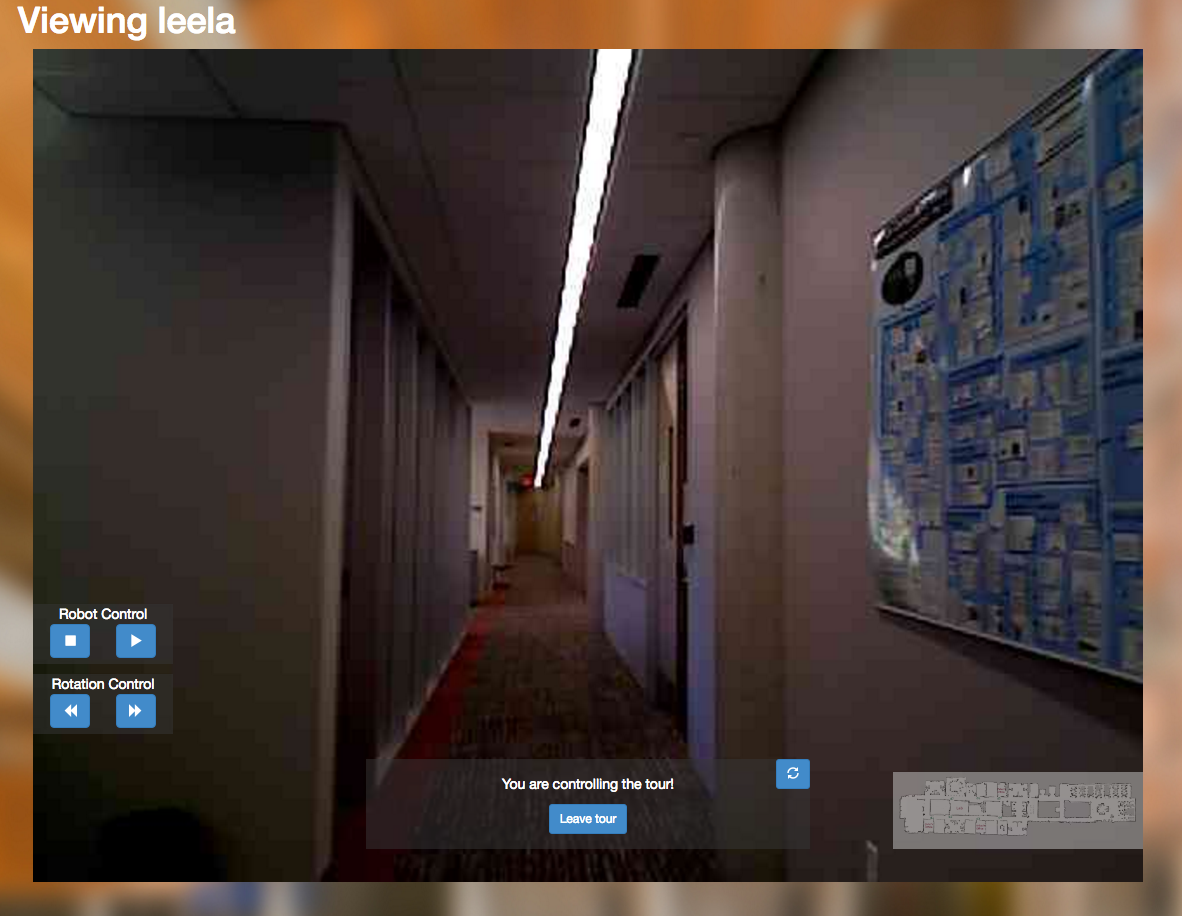
\includegraphics[width=3in]{leader_ui}
\caption{The controls available to the leader}
\end{figure}

The leader UI adds a number of components to that allow the user to
control the operations of the robot. The current list of available capabilities
is as follows

\begin{itemize}
  \item Rotate the robot's base
  \item Navigate to a room on the same floor
  \item Navigate to a door on the same floor
  \item Speak a message (using text-to-speech)
  \item Deliver a spoken message (using text-to-speech) to a location
  \item Pause and resume a scavenger hunt task
  \item Move the robot's camera (on supported robots)
\end{itemize}

\begin{figure}
\centering
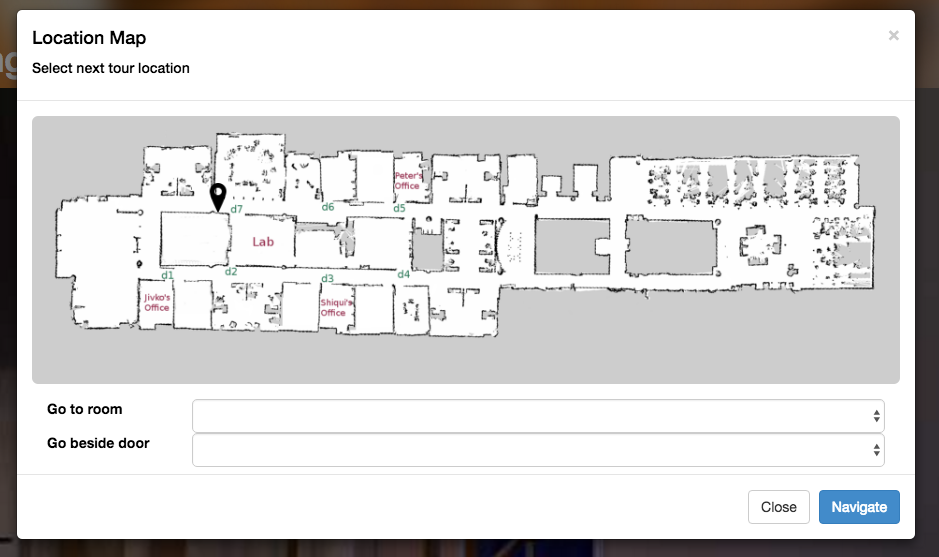
\includegraphics[width=3in]{nav_ui}
\caption{Navigation interface for leaders}
\end{figure}

The user can interact with the interface to request any of the previously
mentioned tasks. For example, whenever the user is the leader a pair of
directional arrow buttons is shown which will immediately rotate the robot when
pressed. Navigation commands are access within the navigation pane

Whenever a user first connects to a robot, the web client will query the robot
for the capabilities that it has (eg: which generation robot, which cameras it
has access to, if the camera has servos, etc...) and then adapt the user
interface accordingly to support whichever robot the user is connected to.

The leader UI was developed using JavaScript and uses sockets to
communicate with the robot. The JavaScript client can interact with ROS via the
socket to make service calls, subscribe and publish to topics, as well as make
actionlib requests. Regardless of the type of the request, it is serialized and
transferred over the socket to be interpreted by the server.

In order to maintain leader consistency, the leader UI will ping the server at
a known interval to ensure the leader is still connected. This allows the
server to become ware of a dropped connection. So if the user closes the window
or the ping fails, the leader will relinquish the leader status so other users
can control robot.


\subsection{Guest UI}

\begin{figure}
\centering
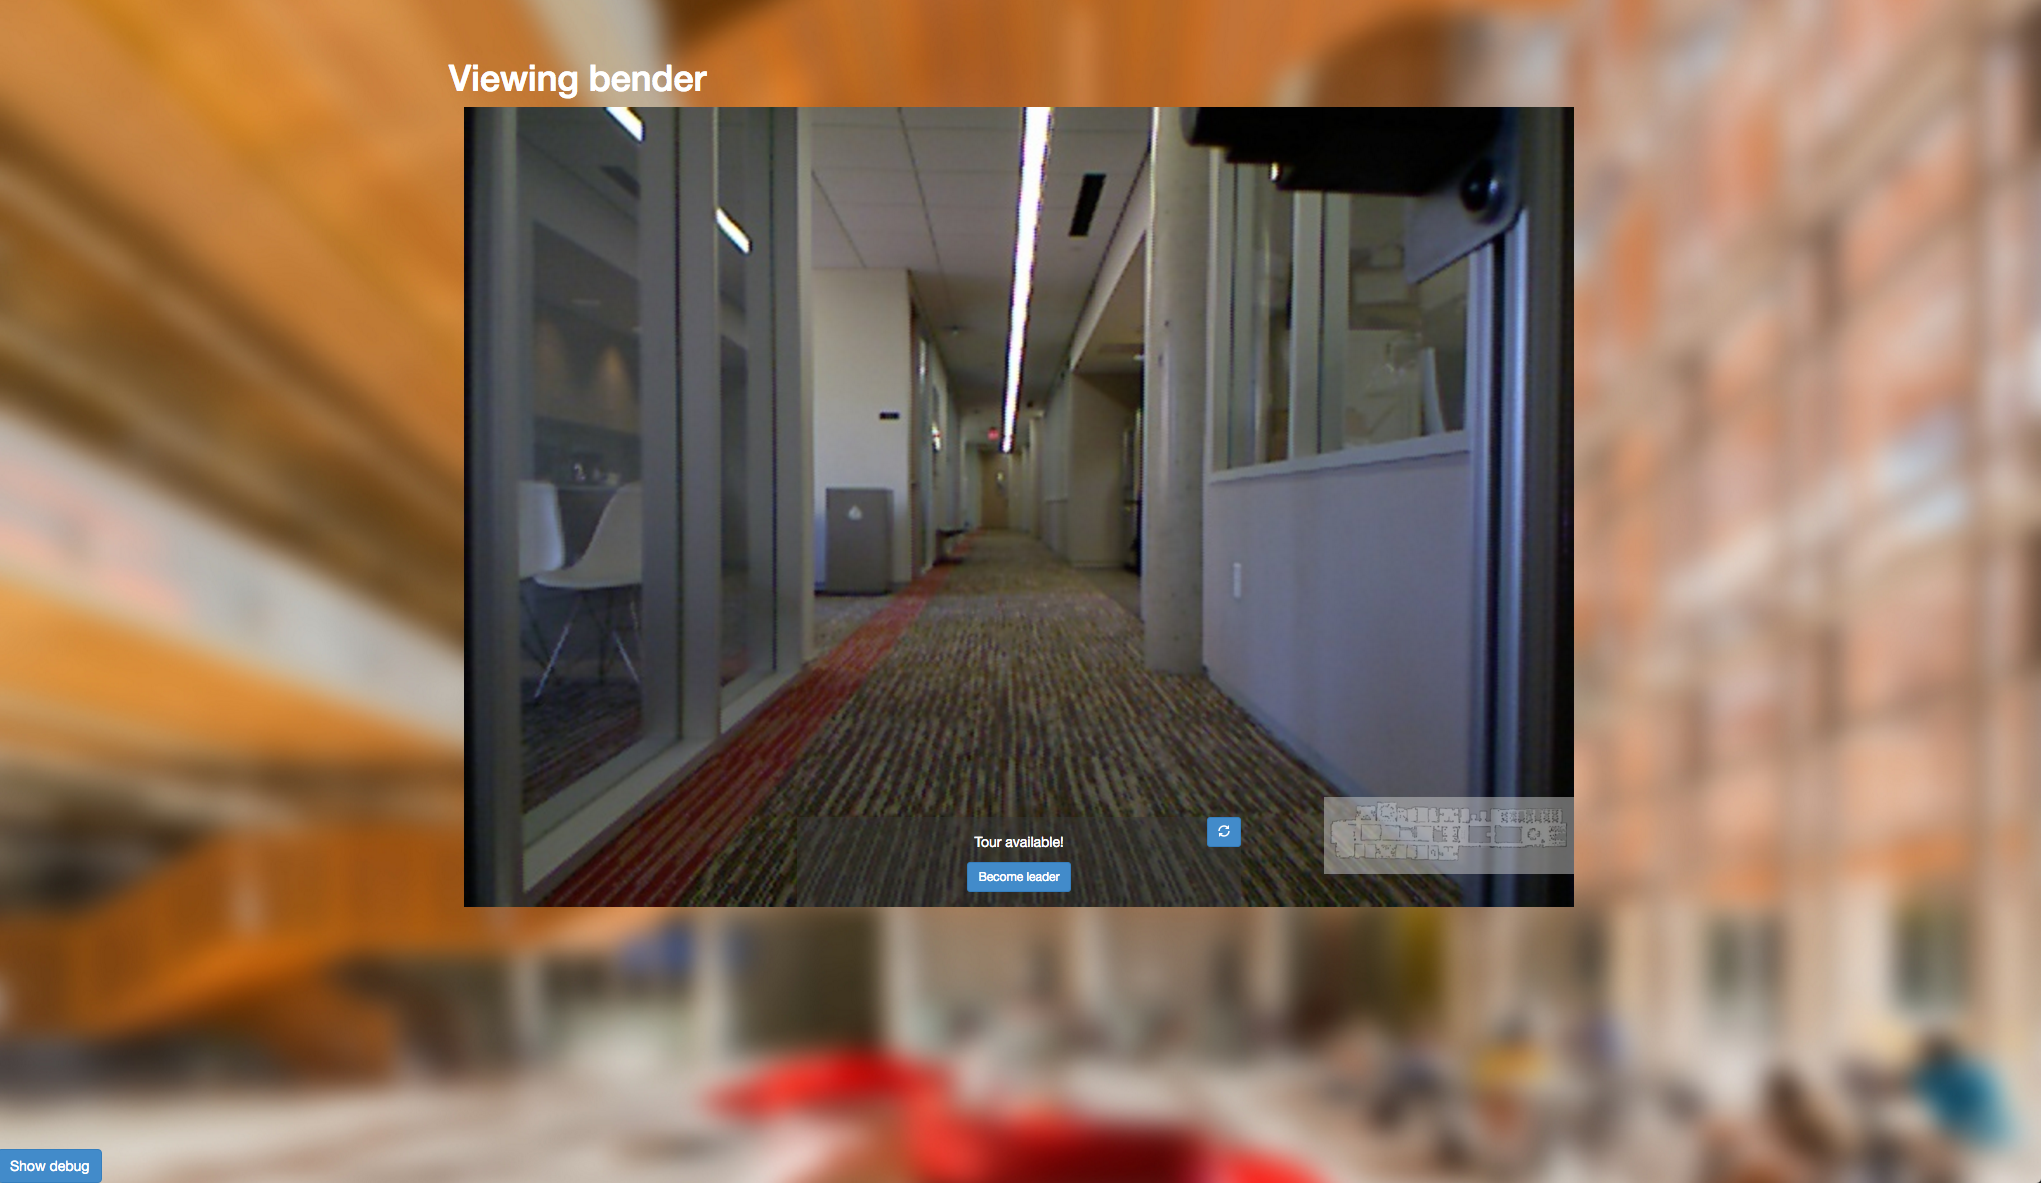
\includegraphics[height=2in]{guestUI}
\caption{What the client sees whenever they are in guest mode}
\end{figure}

The guest UI is the default interface presented to the user whenever he or she
connects to a robot. It dominated by the live stream from the robot's camera
which is shown prominently in the center. The robot's camera is placed in a
position on the robot that makes the user experience feel like a point of view
camera. This makes the experience more immersive and the tour more engaging.

Furthermore, the interface also displays a mini map of which ever floor the
robot is on, with a position marker to indicate the robot's current position.
This map is updated whenever the robot switches floors (via the elevator) to
show the most up to date map of the current floor.

Finally, the guest UI has a status box which displays whether or not a tour is
on-going, allowed, or disabled. From here the user can request to become tour
leader (if available), or wait for a tour to be available.

All our robots support the guest UI during all times we are running them, so
that users can remotely connect to the robots and experience what they are
doing.

\section{Security and Safety}

Security was a top concern since virtour allows external parties to remotely
operate our robots. Our two main security concerns were to prevent unapproved
interactions with the robots and to prevent unauthorized access to virtour.
Furthermore, since the robots are physically navigating potentially crowded
spaces, we wanted to make sure that safety was our number one guarantee.

\subsection{Client Side}

The client works to prevent unapproved interactions by only presenting the user
with ability to interact with the robot in the approved manners. On the
JavaScript client-side, we also only create service and action clients (the
communication methods that are used to request actions on the robot) that
perform specific tasks, rather than general-purpose clients. Each client is
assigned a universally unique identifier (UUID) which is used to authenticate
all communication with the robot.

To ensure the safety of users, the client only provides the user with the
ability to perform two potentially hazardous operations: rotate and navigate.
Both of these operations are moderated server side to ensure that safety is
always maintained.

\subsection{Server Side}

For security reasons, we only allow outside parties to become leaders (and thus
have control of the robot's operations) if we explicitly enable virtual tours
on the robot. Unlike the guest UI which is enabled any time the robot running,
the server implementation of leader control is enabled by default to prevent
unexpected access. Furthermore, all operations which affect the state of the
robot (ie: rotating and navigating) require proper authentication. The server
keeps track of the UUID of the currently active leader, and will only grant
that specific client the ability to control the robot. This prevents
unauthorized users from executing arbitrary actions on the robot. To prevent
denial of service by any one leader (by not relinquishing their leadership or
dropping the connection), the server uses the ping system to ensure that the
leader is alive and connected, as well as an established timeout to prevent any
one valid leader from preventing others from becoming leader.

Safety for users and the robot is provided through the use of shared autonomy.
Whenever users request navigation to locations via the client UI, the robot
will perform the navigation using the full navigation stack which includes the
global obstacle planning and local obstacle avoidance. Furthermore, the server
has a whitelist (which is equal to the list of locations the users can request
on the client) which it uses to verify all navigation requests, to prevent
navigation to unauthorized locations. Finally, because of the way rotation is
implemented, the robot stays entirely within its footprint when it rotates.
When combined with the safety of our navigation stack, this means that in-place
rotation is always safe.


\section{The Server}

\begin{figure}
\centering
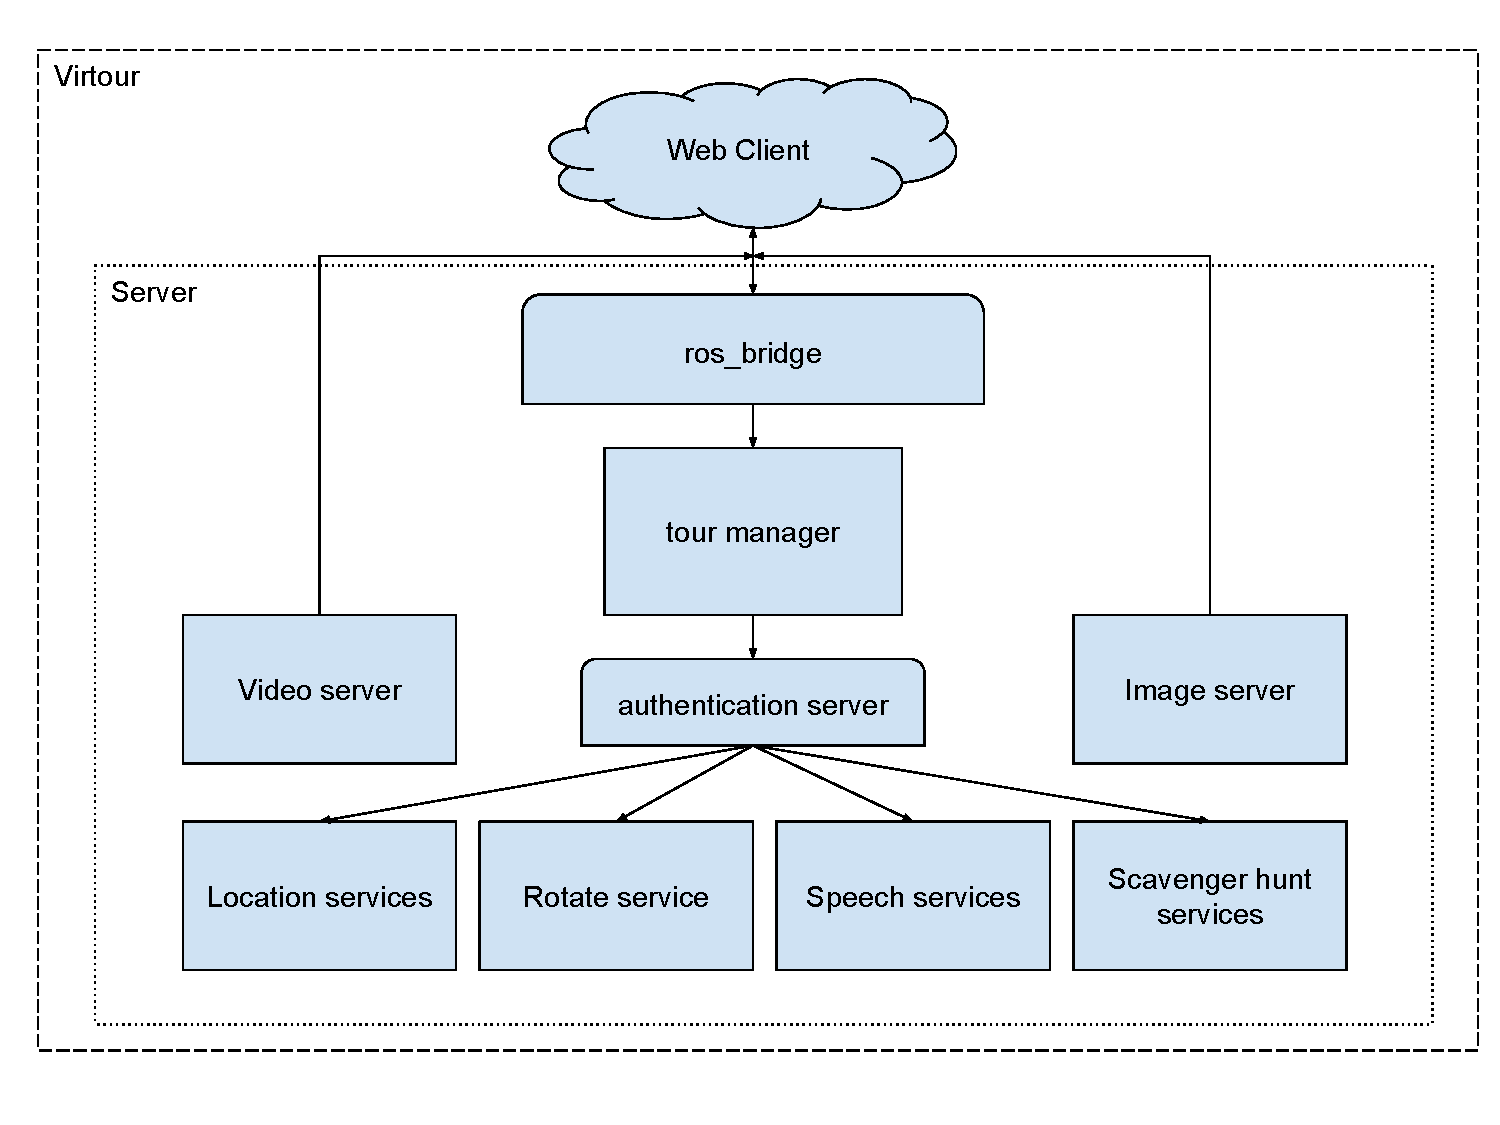
\includegraphics[width=3in]{virtour_server}
\caption{Overview of the virtour server structure and hierarchy}
\end{figure}

The server consists of a number of components which run on the physical robot
to enable the web client to perform the required operations. All communications
from the web client go through the \verb|ros_bridge| node, which is responsible
for translating the serialized socket commands to normal ROS commands. From
there, all requests are sent to the tour manager, which will authenticate the
requests (to ensure they are validly formed and come from an accepted source)
and then triage them to their respective service providers.

\subsection{Tour Manager}

The tour manager serves the role of maintaining tour integrity and managing
active connections with all the clients that are connected to the robot. It
keeps track of an internal state machine which controls whether tours are
enabled and if so whether they are active. It will also maintain connection
with the tour leader through pings to ensure the leader remains alive. If the
leader disconnects (by closing the page) or is disconnected (missing a ping),
the tour manager will demote them and open up the tour again. The tour manager
will also grant tour leader status to clients that properly request it whenever
tours are enabled.

\subsubsection{Authentication}

Due to the open nature of virtour (anyone can access/control our robots),
security became an important factor.User authentication is done by generating a
unique identifier to each client connected (generation is done client-side).
This identifier is used to keep track of all the clients and the leader. All
requests which control robot (ie: navigating, rotating, delivering messages) go
through the authentication server. This verifies that the request is properly
created, is coming from a valid leader, and is being executed at a time when
tours are enabled. There is a 15 minute limit per leader, to avoid
a single leader taking control of the system. Finally, we always have the
option to disable tours (via the tour manager) which will immediately evict any
active leaders and restore control of the robot.

\subsubsection{Robot Control}

The server-side code powering the remote robot control consist of various
service providers which use the tour manager to authenticate requests, and then
triage them to the appropriate robot commands. For example, the rotate control
will take the rotate command (if properly authenticated) and then translate it
to raw segway base navigation commands, which is considered safe because
rotation stays within the robot's footprint so we do not need to consider
obstacle avoidance. However, obstacle avoidance is very important whenever we
are navigating to rooms or doors. For this reason, all navigation commands will
go to the logical planner in the form of ASP goals. For example a request to
navigate to a specific office will be turned into an ASP goal such that it is
impossible for the robot to not be in that location. The navigation and
planning stack then take over and will perform the planning and navigation
required to accomplish the goal.

\subsection{IP management}

In order to manage the IP addresses of all the robots, we created smallDNS
\footnote{Source code is available at \url{https://github.com/pato/smallDNS}}
(small multi-agent locally listable DNS). SmallDNS keeps track of the IP
addresses of each of the robots (which are assigned via DHCP and are thus
variable). Furthermore, it also keeps track of which robots are available and
running via series of pings. This means that the end user does not need to
worry about the IPs of the robots or which ones are alive. So when the user
visits the home page (figure 3), they will see the list of currently active
robots and will be able to connect to each without having to know the IP
address.

SmallDNS consists of a simple DNS server running on our master server, which is
accessible from all our robots. The server was written on python and serves and
handles requests over HTTP. It can handle update requests whenever a robot has
a new IP address, as well as conventional GET requests to display the list of
robots over text or JSON. It stores everything in-memory for performance
reasons, but will write it to disk occasionally to support recovery.

Each of the robots has a bash script which checks the robot's IP address against the
last update IP address to see if there is a change. If the IP has changed, the robot
will perform an update request on the server to inform it of the new address. This
script is configured using a cronjob which runs every three minutes.

\section{Scavenger Hunt Integration}

\begin{figure}
\centering
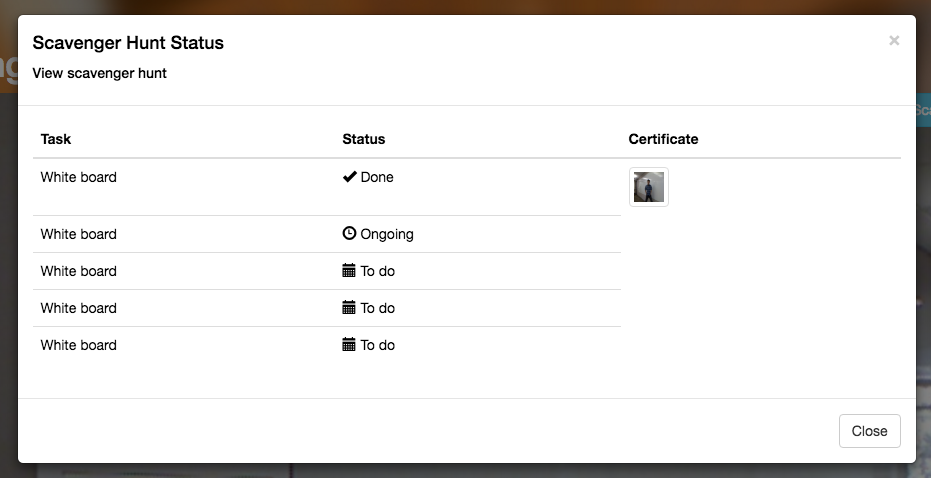
\includegraphics[width=3in]{scav_certs}
\caption{Screenshot of scavenger hunt task status and certificate display}
\end{figure}

Intro about scavenger hunt.

Whenever a user connects to a robot running the scavenger hunt, virtour will
additionally allow the users to interact with the scavenger hunt. For example,
the user can see the list of the currently running tasks by clicking on the
scavenger hunt button. Furthermore, if a task is completed virtour will use its
image web server to display the certificate on the website (appears as a
thumbnail but is expanded whenever clicked on). Finally, if the user is the
leader, they can also control the operation of scavenger hunt by stopping and
resuming the current task. This allows a user can stop the current scavenger
hunt task, then navigate the robot elsewhere or perform any other supported
operation, and resume the scavenger hunt later.

\section{Conclusions and Future Work}

In this paper we introduced a novel telepresence system which gives users
shared autonomy over the control of our robots. This system allows users to use
their common internet-powered devices to access the virtour website. The
virtour website allows users to securely join an existing tour as spectators,
or, if available, to optionally lead a tour. This would give them the ability
to make the robot navigate to desired locations and doors, as well as deliver
messages, or perform scavenger hunt tasks. Users can experience the tour
through the on-board camera which is streamed dynamically to the website as
well as to track the robot's movement using the real-time map.

However, there is still work left in building a more complete virtual tour
system. Further work could extend the navigation system to allow the users
point-and-click navigation to arbitrary points, while still maintaining shared
autonomy. There is also work in adding more ways for remote users to interact
with the robot's environment, such as using actuators or interacting via a
mounted arm on the robot. There are multiple other ways of improving the client
user interface such as adding the display of other information such as distance
traveled or battery level information.

Finally, although our focus has been on remotely operated building tours,
virtour has laid the groundwork for a more complete telepresence robot system
which could target other commercial uses such as hospitals (for family visits,
or nurse checkups), as well other research-oriented projects such as HRI
studies or robot monitoring systems. Most of our work is directly applicable
and can be tailored to many different uses, since the communication,
authentication, and interaction protocols that virtour uses can be independently
used.

\section{Acknowledgments}

Virtour couldn't have been completed with the help and support of my original
research educator Matteo Leonetti, and my current research educator Jivko
Sinapov. Thank you to Peter Stone for providing direction and for all his
support. Thanks to Shiqi Zang for helping and me with the scavenger hunt
integration. Finally, thank you to Maxwell Svetlik for insightful comments and
help through the project, Walter Sagehorn for helping develop smallDNS and to
Benjamin Singer for developing the message delivery tasks.

\nocite{*}
\bibliographystyle{apacite}
\bibliography{citations}
    
\end{document}
